% !TeX root = ../apuntes-ea.tex


\chapter{Homomorfismos de grupos}

\section{Homomorfismos de grupos}

\begin{dfn}[Homomorfismo de grupos]
	Sean $(G_1, \cdot), (G_2, \ast)$ grupos. Decimos que $f: G_1 \to G_2$ es un homomorfismo de grupos si $\forall a,b \in G_1,\ f(a\cdot b) = f(a) \ast f(b)$.

	\begin{itemize}
		\item si $f$ es inyectiva, $f$ es un monomorfismo
		\item si $f$ es sobreyectiva, $f$ es un epimorfismo
		\item si $f$ es biyectiva, $f$ es un isomorfismo
		\item si $G_2 = G_1$ y $f$ es un isomorfismo, entonces $f$ se llama automorfismo
	\end{itemize}
	Si existe un isomorfismo entre dos grupos, decimos que son isomorfos y lo denotamos por $G_1 \isom G_2$.
\end{dfn}

\begin{figure}[h]
	\centering
	\begin{tikzpicture}[scale=0.7]
	\node (a) at (0,1) {$a$};
	\node (b) at (0,0) {$b$};
	\node (ab) at (0,-1) {$a\ast b$};
	
	\node (fa) at (4,1) {$f(a)$};
	\node (fb) at (4,0) {$f(b)$};
	\node (fab) at (4,-1) {$f(a)\ast f(b)$};
	\draw (0,0) ellipse (.9 and 2);
	\draw (4,0) ellipse (1.8 and 2);
	
	\draw (0, -2) node[anchor=north] {$G_1$};
	
	\draw (4, -2) node[anchor=north] {$G_2$};
	
	\draw[-{Latex[length=2mm]}] (a) -- (fa);
	\draw[-{Latex[length=2mm]}] (b) -- (fb);
	\draw[-{Latex[length=2mm]}] (ab) -- (fab);
	\end{tikzpicture}
	\caption{Homomorfismo de grupos}
	\label{fig:homomorfismo}
\end{figure}


\begin{dfn}[Núcleo de un homomorfismo]
	Sea $f:G_1 \to G_2$ un homomorfismo. Definimos el núcleo $\ker f = \{x \in G_1 \mid f(x) = e_2 \in G_2\}$ (los que van a parar al neutro).
\end{dfn}

\begin{dfn}[Imagen de un homomorfismo]
	Sea $f:G_1 \to G_2$ un homomorfismo. Definimos la imagen $\ima f = \{y \in G_2 \mid \exists x \in G_1, f(x) = y\}$.
\end{dfn}

\begin{pro}Sea $f: G_1 \to G_2$ un homomorfismo. $\ker f < G_1$.
\end{pro}

\begin{proof} Probamos las 3 propiedades de los subgrupos
	\begin{enumerate}
		\item $a,b \in \ker f \implies a \cdot b \in \ker f$. $f(a \cdot b) = f(a) \ast f(b) = e_2 \ast e_2 = e_2$.
		\item $a \in \ker f \implies a^{-1} \in \ker f$. $f(a) = e_2,\ f(a^{-1}) = e_2 \implies (f(a))^{-1} = e_2$.
		\item $e_1 \in \ker f$.
	\end{enumerate}
\end{proof}

\begin{thm}
	Sea $f: G_1 \to G_2$ un homomorfismo. $\ima f < G_2$.
\end{thm}

\begin{proof} Es análoga a la del $\ker f$.\end{proof}

\begin{thm}
	Sea $f : G_1 \to G_2$ un homomorfismo. $\ker f \normsub G_1$
\end{thm}

\begin{proof}
	Tenemos que probar que $\forall a \in G_1, a (\ker f) a^{-1} \subset \ker f$.
	
	Sea $h \in \ker f$. $f(a h a^{-1}) = f(a)\underbrace{f(h)}_{e_2}f(a^{-1}) = f(a)f(a^{-1}) = e_2\subset \ker f$
\end{proof}

\begin{pro}
	Sea $f:G_1 \to G_2$ un homomorfismo de grupos. $f$ es inyectiva si y solo si $\ker f = \{e\}$.
\end{pro}

\begin{proof}$ $ \newline
	\begin{itemize}
		\item $(\impliedby$) Suponemos que $f$ es inyectiva. Sabemos que en un homomorfismo $f(e_1) = e_2$ y además $\ker f = {e_1}$ por hipótesis.
		\item $(\implies)$ Tenemos que probar que dados $a,b \in G_1,\ f(a) = f(b) \implies a = b$. Decir que $f(a) = f(b)$ es lo mismo que decir $e_2 = f(a)^{-1}f(b) = f(a^{-1}) f(b) = f(a^{-1}b) \implies a^{-1}b \in \ker f = \{e_1\} \implies a = b$.
	\end{itemize}
\end{proof}

\begin{pro}
	Sean $G_1, G_2, G_3$ grupos y sean $f:G_1 \to G_2,\ g:G_2 \to G_3$ homomorfismos de grupos. Entonces $g \circ f$ es a su vez un homomorfismo de grupos.
\end{pro}

\begin{thm}
	Sea $f:G_1 \to G_2$ un homomorfismo de grupos. Entonces $o(f(g))$ divide a $o(g)$.
\end{thm}

\begin{thm}
	Sea $f:G_1 \to G_2$ un isomorfismo de grupos. Entonces $o(g) = o(f(g))$.
\end{thm}

\begin{proof}
	Consideramos $f$ y $f^{-1}$ para los que se verifica el teorema anterior. $o(g) \mid o(f(g)) \land o(f(g)) \mid o(f^{-1}(f(g))) = o(g) \implies o(g) = o(f(g))$. 
\end{proof}

%20180925

\section{Retículo de subgrupos}

\begin{dfn}[Retículo de subgrupos]
	Dado un grupo $G$, el retículo de subgrupos es un grafo con todos los subgrupos de $G$. Denotamos la relación de inclusión con un vértice entre dos grupos. Es costumbre poner el mayor grupo arriba y denotar la inclusión por las diferencias en altura.
\end{dfn}

Lo importante de esta sección:
\begin{itemize}
	\item Todo subgrupo de un grupo cíclico es cíclico.
	\item Dado un epimorfismo entre dos grupos existe una correspondencia biyectiva entre los subgrupos del primero y los del segundo.
	\item En $\ZnZ$ existe un subgrupo por cada divisor de $n$ y esos son todos los subgrupos que hay.
\end{itemize}

\begin{ej}[Retículo de subgrupos $\Z$]
	$\Z$ tiene infinitos subgrupos, todos los $k\Z$. En muchas ocasiones nos va a interesar solo dibujar unos pocos, para relacionarlos con subgrupos de otros grupos distintos de $\Z$. A continuación se muestra el retículo de subgrupos de $\Z$ construido a partir de $6\Z$.
	
	\begin{figure}[h]
		\centering
		\begin{tikzpicture}
		\node (z) at (0,1) {$\Z$};
		\node (2z) at (-1,0) {$2\Z$};
		\node (3z) at (1,0) {$3\Z$};
		\node (6z) at (0,-1) {$6\Z$};
		
		\draw (z) -- (2z);
		\draw (z) -- (3z);
		\draw (2z) -- (6z);
		\draw (3z) -- (6z);
		\end{tikzpicture}
		\caption{Una parte del retículo de subgrupos de $\Z$, en concreto la de los $n\Z$ con $n \divides 6$.}
	\end{figure}

	Los grupos que contienen a $6\Z$ son los de la forma $k\Z$ donde $k$ divide a $6$, ya que entre los múltiplos de los divisores de $6$ también se encuentran los múltiplos de $6$.
\end{ej}

\begin{pro}
	Sea $n = \min_{r \in \N,\\r > 0} \{ r \in H,\ H < \Z\}$. Entonces $nH = \Z$.
\end{pro}
\begin{proof}
	Probamos la doble inclusión. Por hipótesis $n \in H$ y por tanto $\langle n \rangle = n\Z \subset H$. Sea $\alpha \in H$. Por el algoritmo de la división, podemos expresar $\alpha = an + s$ con $0 \leq s < n \implies s = 0 \implies H \subset n\Z$. Luego $H = n\Z$.
\end{proof}

El siguiente teorema no lo ha dado Orlando explícitamente pero básicamente lo que dice es lo que dijo en las 3 clases sobre correspondencia entre subgrupos pero un poco más ordenado.

\begin{thm}[de correspondencia entre subgrupos mediante homomorfismos]
	Sea $f:G_1 \to G_2$ un homomorfismo de grupos. Se tiene \cite{dor96}:
	\begin{enumerate}
		\item Si $H_1 < G_1$ entonces $f(H_1) < G_2$
		\item Si $H_2 < G_2$ entonces $f^{-1}(H_2) = \{h_1 \in G_1 \mid f(h_1) \in H_2\} < G_2$
		\item Si $H_2 \normsub G_2$ entonces $f^{-1}(H_2) \normsub G_1$
		\item Si $H_1 \normsub G_1$ y $f$ es además sobreyectiva (es un epimorfismo) entonces $f(H_1) \normsub G_2$
	\end{enumerate}
\end{thm}

\begin{proof}$ $\newline
	\begin{enumerate}
		\item Demostramos que se cumplen las 3 propiedades de los grupos. Sabemos que $e_1 \in H_1 \implies e_2 \in f(H_1) = H_2$. Además, sabemos que $\forall x \in H_1,\ \inv{x} \in H_1$ y por ser $f$ un homomorfismo tenemos que $\forall f(x) \in H_2,\ \inv{f(x)} = f(\inv{x}) \in H_2$. Por último, tenemos que $\forall x,y \in H,\ xy \in H_1 \implies \forall f(x),f(y) \in H_2,\ f(x)f(y) = f(xy) \in H_2$.
		\item Es análoga a la de la primera afirmación.
		\item Tenemos que probar que para un $g_1 \in G_1,\ \forall h_1 \in f^{-1}(H_2) = H_1,\ g_1 h_1 = h_1 g_1$. Sabemos que $\forall h_1,\ \exists h_2 \in H_2 \mid \inv{f}(h_2) = h_1$. Entonces $g_1h_1 = h_1 g_1 \iff \inv{f}(g_2)\inv{f}(h_2) = \inv{f}(h_2)\inv{f}(g_2) \iff \inv{f}(g_2h_2) = \inv{f}(h_2g_2)$ que es cierto por hipótesis de que $H_2$ es normal.
		\item Tenemos que probar que para $g_2 \in G_2$ dado, $\forall h_2 \in H_2 = f(H_1),\ g_2h_2 = h_2g_2$. Comenzamos por asegurar que $\exists g_1 \in G_1 \mid f(g_1) = g_2$ por ser $f$ sobreyectiva. Por tanto $g_2h_2 = h_2 g_2 \iff f(g_1)f(h_1) = f(h_1)f(g_1) \iff f(g_1h_1) = f(h_1g_1)$ que es cierto por hipótesis.
	\end{enumerate}
\end{proof}

Queremos establecer una relación entre los retículos de subgrupos de dos grupos que son el dominio y la imágen de un epimorfismo $f: G_1 \to G_2$. Los subgrupos de $G_2$ siempre contendrán al elemento neutro $e_2$ por lo que podemos establecer una relación natural entre los subgrupos de $G_1$ que contienen a $\ker f$ con los subgrupos de $G_2$.

\begin{thm}\footnote{Este teorema es un desastre. Las hipótesis no las ha dado y las conclusiones tampoco. Es lo que más o menos he creido que quería decir. Es posible que se corresponda con la proposición 4.4.6 del \cite{dor96} pero en dicha proposición no se exige que $f$ sea sobre.}
	Sea $f: G_1 \to G_2$ un epimorfismo. Existe una biyección entre el retículo de subgrupos de $G_2$ y subgrupos de $G_1$ que contienen al $\ker f$. Se cumple que $H_2 < G_2 \iff \inv{f}(H_2) \supset \ker f$.
	
	En particular, el número de subgrupos de $G_2$ es igual al número de subgrupos de $G_1$ que contienen al núcleo.
	\begin{align*}
		|\{H_2 \mid H_2 < G_2\}| = |\{H_1 < G_1 \mid \ker f \in H_1\}|
	\end{align*}
\end{thm}

\begin{proof}
	Sabemos que por ser $f$ homomorfismo, $H_1 < G_1 \implies f(H_1) < G_2$.
	
	Veamos que la relación entre los subconjuntos de $G_1$ y de $G_2$ se mantiene al aplicar el epimorfismo. Sea $H_2 \subset G_2$. Como $f$ es sobre $f(\inv{f}(H_2)) = H_2$. Ahora sea $H_2' \mid H_2 \subset H_2' \subset G_2$. Ocurre lo de antes y además $\inv{f}(H_2) \subset \inv{f}(H_2') \subset G_1$.
	
	Ahora lo extendemos de subconjuntos a subgrupos. Asociamos a cada $H_2 < G_2$ el subgrupo $\inv{f}(H_2) < G$. Es un subgrupo porque al ser $f$ epimorfismo mantiene la operación. En particular, $e_2 \in H_2 \implies \ker f = \inv{f}(e_2) \subset \inv{f}(H_2)$.
	
	Por último afirmamos que si $\ker f \subset H_1 < G_1$, entonces $H_1 = \inv{f}(f(H_1))$. Para probar esto probamos la doble inclusión. $H_1 \in \inv{f}(f(H_1))$ es evidente pues $h \in H_1 \implies f(h) \in f(H_1)$. Ahora probamos $\ker f \subset H_1 \implies H \subset \inv{f}(f(H_1))$.
	\begin{align*}
		\alpha \in \inv{f}(f(H_1)) \iff& f(\alpha) \in \inv{f}(f(H_1)) \\
		\iff& \exists h_1 \in f(H_1) \mid f(\alpha) \in f(H_1) \\
		\iff& \exists h_1 \in H \mid f(\alpha)\inv{(f(h_1))} = e_2 \\
		\iff& \exists h_1 \in H_1 \mid f(\alpha \inv{h_1}) = e_2 \\
		\iff& \exists h_1 \in H_1 \mid \alpha \inv{h_1} \in \ker f \\
		&\alpha \inv{h_1} h_1 \implies \alpha \in H_1
	\end{align*}
\end{proof}

\begin{figure}[h]
	\centering
	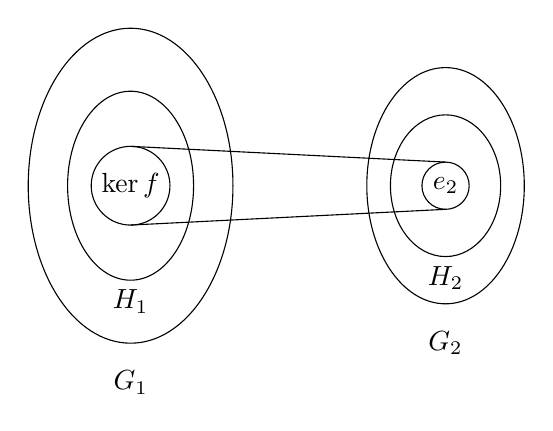
\begin{tikzpicture}
		\draw (-2,0) ellipse (1.3 and 2);
		\draw (2, 0) ellipse (1 and 1.5);
		\draw (-2,-2.5) node {$G_1$};
		\draw (2, -2) node {$G_2$};
		
		\node (ker) at (-2, 0) {$\ker f$};
		\node (e2) at (2,0) {$e_2$};
		
		\draw (ker) ellipse(.5 and .5);
		\draw (e2) ellipse (.3 and .3);
		\draw (-2,.5) -- (2,.3);
		\draw (-2,-.5) -- (2,-.3);
		
		% subgrupos de G1
		\draw (ker) ellipse (.8 and 1.2);
		\draw (-2,-1.2) node[anchor=north] {$H_1$};
		
		% subgrupos de G2
		\draw (e2) ellipse (.7 and .9);
		\draw (2, -.9) node[anchor=north] {$H_2$};
	\end{tikzpicture}
\end{figure}

\section{Teoremas de la isomorfía (versión de clase)}

\begin{pro}[O ejemplo]
	Sea $f: \ZnZ \to \ZnZ$. $f$ es un isomorfismo $\iff f(\overline{1}) = \overline{a} \in \uds{\ZnZ}$
\end{pro}

\begin{ej}
	Sea $g \in G$ fijado. Definimos $\phi_g : G \to G$
	\begin{align*}
		G \to^{\phi_g} & G \to^{\phi^{-1}_g} & G \\
		x \mapsto &gx\inv{g} & \\
		&z \mapsto &\inv{g}x\inv{(\inv{g})}
	\end{align*}
	Y $\phi_g \cdot \phi_g^{-1} = Id$.
\end{ej}

\begin{proof}
	Para que $f$ sea isomorfismo tiene que ser sobre luego $o(\overline{a}) = n \implies \overline{a} \in \uds{\ZnZ}$.
\end{proof}

\begin{thm}
	\label{teorema:preisomorfia1}
	Sea $f: G_1 \to G_2$ un homomorfismo de grupos, $H \normsub G_1$ con $H \subset \ker f$. Sea $\pi: G_1 \to G_1/H$ el homomorfismo que genera las clases de equivalencia (ver figura \ref{fig:tmisomorfia1}). Entonces se cumple lo siguiente
	\begin{enumerate}
		\item existe un homomorfismo de grupos $\overline{f}:G_1/H \to G_2$ tal que $\overline{f} \circ \pi = f$
		\item $\ker \overline{f} = \ker f / H$
	\end{enumerate}
\end{thm}

\begin{figure}[h]
\centering
\begin{tikzpicture}
\node (g1) at (0,0) {$a \in G_1$};
\node (g2) at (4,0) {$f(a) \in G_2$};
\node (gh) at (0, -3) {$\overline{a} \in G_1/H$};

\draw[-{Latex[length=2mm]}] (g1) -- (g2) node[pos=.5, above] {$f$};
\draw[-{Latex[length=2mm]}] (g1) -- (gh) node[pos=.5, left]{$\pi$};
\draw[-{Latex[length=2mm]}] (gh) -- (g2) node[pos=.5, below] {$\overline{f}$};
\end{tikzpicture}
\caption{Homomorfismos que intervienen en el teorema \ref{teorema:preisomorfia1}}
%TODO
\label{fig:otracosa}
\end{figure}

\begin{proof} $ $\newline
	\begin{enumerate}
		\item Probaremos que si construimos $\overline{f}$ con $\overline{f}(\overline{a}) = f(a)$ entonces $\overline{f}$ está bien definida. Tenemos que ver que $\overline{a} = \overline{a'} \implies f(a) = f(a')$. Partimos de $\overline{a} = \overline{a'} \implies a \inv{(a')} \in H \implies f(a \inv{(a')}) = e_2 \implies f(a) \inv{f(a')} = e_2 \implies f(a) = f(a')$.
		
		\item Observemos que $\overline{f}(\overline{a}\overline{b}) = \overline{f}(\overline{ab}) = f(ab) = f(a)f(b)=\overline{f}(\overline{a})\overline{f}(\overline{b})$. Ahora probamos las dos inclusiones a la vez $\overline{a} \in \ker \overline{f} \iff \overline{f}(\overline{a}) = e_2 \iff f(a) = e_2 \iff \overline{a} \in \ker f$.
	\end{enumerate}
\end{proof}

\begin{thm}[Primer de la isomorfía]
	Sea $f:G_1 \to G_2$ un epimorfismo. Existe un isomorfismo $\overline{f}: G_1 / \ker f \to G_2$.
\end{thm}

\begin{figure}[h]
	%TODO hacer
	\centering
	\begin{tikzpicture}
	\node (g1) at (0,0) {$G_1$};
	\node (g2) at (4,0) {$G_2$};
	\node (gh) at (0, -3) {$G_1/\ker f$};
	
	\draw[-{Latex[length=2mm]}] (g1) -- (g2) node[pos=.5, above] {$f$};
	\draw[-{Latex[length=2mm]}] (g1) -- (gh) node[pos=.5, left]{$\pi$};
	\draw[-{Latex[length=2mm]}] (gh) -- (g2) node[pos=.5, below] {$\overline{f}$};
	\end{tikzpicture}
	\caption{Primer teorema de la isomorfía.}
	\label{fig:tmisomorfia3}
\end{figure}

\begin{proof}
	$f = \pi \circ \overline{f}$ y $f$ es sobre, luego $\overline{f}$ también es sobreyectiva.
	
	% TODO probar que f barra es inyectiva \implies es isomorfismo
\end{proof}

\begin{thm}[Segundo teorema de la isomorfía]
	
	Sean $H \normsub G,\ K \normsub G$ y $H \subset K$ Entonces
	\begin{align}
		(G/H)/(K/H) = G/K
	\end{align}
\end{thm}

\begin{figure}[h]
	%TODO hacer
	\centering
	\begin{tikzpicture}
	\node (g1) at (0,0) {$G$};
	\node (g2) at (4,0) {$G/K$};
	\node (gh) at (0, -3) {$G/H$};
	
	\draw[-{Latex[length=2mm]}] (g1) -- (g2) node[pos=.5, above] {$h$};
	\draw[-{Latex[length=2mm]}] (g1) -- (gh) node[pos=.5, left]{$\pi$};
	\draw[-{Latex[length=2mm]}] (gh) -- (g2) node[pos=.5, below] {$\overline{h}$};
	\end{tikzpicture}
	\caption{Segundo teorema de la isomorfía.}
	\label{fig:tmisomorfia2}
\end{figure}

\begin{proof}
	$\overline{h}$ es sobreyectiva y $\ker \overline{h} = K/H$
\end{proof}

% 20180927

\begin{thm}
	Sea $f:G_1 \to G_2$ un epimorfismo. Si $N \normsub G_1$, entonces $f(N) \normsub G_2$. Como $f$ es epimorfismo cualquier $g \in G_2,\ g_2 = f(g_1)$ para algún $g_1 \in G_1$. Como $N \normsub G_1$, tenemos que $gN\inv{g} \in N$. Que $f(N) \normsub G_2$ quiere decir que $\forall f(g) \in G_2, f(g)f(N)f(\inv{g}) \subset f(N)$. Ahora bien $f(g)f(N)\inv{f(g)}$. Y esto sigue pero lo ha dicho y no lo ha escrito y no me ha dado tiempo.
\end{thm}

\begin{lem}
	Sea $h:G_1 \to G_2$ homomorfismo de grupos. Sean $N \normsub G_1$ y $N \subset \ker h$. 
	\begin{enumerate}
		\item Entonces existe un homomorfismo de grupos $\overline{f}:G_1/N \to G_2$ que cumple $\overline{f} \circ \pi = f$
		\item $\ker \overline{f} = \ker f / N$.
	\end{enumerate}
\end{lem}

\begin{cor}
	Si $N = \ker f$ entonces $\ker \overline{f} = \{0\}$ y $\overline{f}$ es un monomorfismo.
\end{cor}

\begin{cor} % TODO esto es el primer teorema otra vez
	Si $f$ es además un epimorfismo, entonces $\overline{f}$ es una biyección.
\end{cor}

% TODO poner aquí la imágen del primer teoremaº



\begin{proof}
	Consideramos $f:H \to HK$ que es un homomorfismo porque $H < HK$ (porque $h = he_k,\ \forall h \in H$ y satisface la definción de producto). Y ahora consideramos un epimorfismo $h:HK \to HK/K$ que existe porque $K \normsub HK$. Sea $\pi = f \circ g$. Afirmamos que $\ker \pi = H \cap K$. Faltan cosas.
	
	\begin{align*}
		H/(H\cap K) \isom HK/K
	\end{align*}
\end{proof}

\begin{cor}
	Si $H,K < G$ con $K \normsub G$ entonces existe un epimorfismo $\pi:H\to HK/K$ y $\ker \pi = H \cap K$.
\end{cor}

\begin{thm}\footnote{Esta vez si que dijo teorema.}
	Sea $f:G_1 \to G_2$ un homomorfismo de grupos. Entonces $\ima f \isom G_1 / \ker f$.
\end{thm}

Este teorema viene a decir que dado un homomorfismo $f:G_1 \to G_2$, si lo restringimos a $f:G_1 \to \ima f$ obtenemos un epimorfismo.

%_---------------

\begin{pro}
	Sea $G$ un grupo con orden $n$. Sea $H < G$ con índice de $H = p \mid mcd(p,n) = 1$. Entonces $H$ es un subgrupo normal.
\end{pro}

\section{Teoremas de la isomorfía (versión con pies y cabeza)}

\begin{thm}(Primer teorema de la isomorfía)
	Sea $f:G_1 \to G_2$ un epimorfismo y sea $\pi:G_1 \to G_1/\ker f$. Entonces existe un isomorfismo $\overline{g} : G_1 / \ker f \to G_2$ tal que $f = \pi \circ \overline{f}$.
\end{thm}

\begin{figure}[h]
	%TODO hacer
	\centering
	\begin{tikzpicture}
	\node (g1) at (0,0) {$G_1$};
	\node (g2) at (4,0) {$G_2$};
	\node (gh) at (0, -3) {$G_1/\ker f$};
	
	\draw[-{Latex[length=2mm]}] (g1) -- (g2) node[pos=.5, above] {$f$};
	\draw[-{Latex[length=2mm]}] (g1) -- (gh) node[pos=.5, left]{$\pi$};
	\draw[-{Latex[length=2mm]}] (gh) -- (g2) node[pos=.5, below] {$\overline{f}$};
	\end{tikzpicture}
	\caption{Primer teorema de la isomorfía.}
	\label{fig:tmisomorfia1}
\end{figure}

\begin{thm}(Segundo teorema de la isomorfía)
	Sea $G$ un grupo, $H \normsub G,\ K \normsub G$ y $H < K$. Entonces $K/H$ es un subgrupo normal de $G/H$ y
	\begin{align}
		\sfrac{G/H}{K/H} \isom G/K
	\end{align}
\end{thm}

\begin{thm}[Tercer teorema de la isomorfía]
	Sea $G$ un grupo, $H < G,\ K \normsub G$. Entonces $HK < G$, $K \normsub HK$ y $H\cap K \normsub H$. Además,
	\begin{align}
		\sfrac{HK}{K} \isom \sfrac{H}{(H \cap K)}
	\end{align}
\end{thm}
